%%%%%%%%%%%%%%%%%%%%%%%%%%%%%%%%%%%%%%%%%
% Arsclassica Article
% LaTeX Template
% Version 1.1 (1/8/17)
%
% This template has been downloaded from:
% http://www.LaTeXTemplates.com
%
% Original author:
% Lorenzo Pantieri (http://www.lorenzopantieri.net) with extensive modifications by:
% Vel (vel@latextemplates.com)
%
% License:
% CC BY-NC-SA 3.0 (http://creativecommons.org/licenses/by-nc-sa/3.0/)
%
%%%%%%%%%%%%%%%%%%%%%%%%%%%%%%%%%%%%%%%%%

%----------------------------------------------------------------------------------------
%	PACKAGES AND OTHER DOCUMENT CONFIGURATIONS
%----------------------------------------------------------------------------------------

\documentclass[
10pt, % Main document font size
a4paper, % Paper type, use 'letterpaper' for US Letter paper
oneside, % One page layout (no page indentation)
%twoside, % Two page layout (page indentation for binding and different headers)
headinclude,footinclude, % Extra spacing for the header and footer
BCOR5mm, % Binding correction
]{scrartcl}

%%%%%%%%%%%%%%%%%%%%%%%%%%%%%%%%%%%%%%%%%
% Arsclassica Article
% Structure Specification File
%
% This file has been downloaded from:
% http://www.LaTeXTemplates.com
%
% Original author:
% Lorenzo Pantieri (http://www.lorenzopantieri.net) with extensive modifications by:
% Vel (vel@latextemplates.com)
%
% License:
% CC BY-NC-SA 3.0 (http://creativecommons.org/licenses/by-nc-sa/3.0/)
%
%%%%%%%%%%%%%%%%%%%%%%%%%%%%%%%%%%%%%%%%%

%----------------------------------------------------------------------------------------
%	REQUIRED PACKAGES
%----------------------------------------------------------------------------------------

\usepackage[
nochapters, % Turn off chapters since this is an article        
beramono, % Use the Bera Mono font for monospaced text (\texttt)
eulermath,% Use the Euler font for mathematics
pdfspacing, % Makes use of pdftex’ letter spacing capabilities via the microtype package
dottedtoc % Dotted lines leading to the page numbers in the table of contents
]{classicthesis} % The layout is based on the Classic Thesis style

\usepackage{arsclassica} % Modifies the Classic Thesis package

\usepackage[T1]{fontenc} % Use 8-bit encoding that has 256 glyphs

\usepackage[utf8]{inputenc} % Required for including letters with accents

\usepackage{graphicx} % Required for including images
\graphicspath{{Figures/}} % Set the default folder for images

\usepackage{enumitem} % Required for manipulating the whitespace between and within lists

\usepackage{lipsum} % Used for inserting dummy 'Lorem ipsum' text into the template

\usepackage{subfig} % Required for creating figures with multiple parts (subfigures)

\usepackage{amsmath,amssymb,amsthm} % For including math equations, theorems, symbols, etc

\usepackage{varioref} % More descriptive referencing

%----------------------------------------------------------------------------------------
%	\frac{d_t(w_1, N_t^1(u) \backslash N_t^1(v)}{|N_t^1(u)| + d_t(w_1, N_t^2(u))} \times \frac{1}{d_t(w_1)} STYLES
%---------------------------------------------------------------------------------------

\theoremstyle{definition} % Define theorem styles here based on the definition style (used for definitions and examples)
\newtheorem{definition}{Definition}

\theoremstyle{plain} % Define theorem styles here based on the plain style (used for theorems, lemmas, propositions)
\newtheorem{theorem}{Theorem}

\theoremstyle{remark} % Define theorem styles here based on the remark style (used for remarks and notes)

%----------------------------------------------------------------------------------------
%	HYPERLINKS
%---------------------------------------------------------------------------------------

\hypersetup{
%draft, % Uncomment to remove all links (useful for printing in black and white)
colorlinks=true, breaklinks=true, bookmarks=true,bookmarksnumbered,
urlcolor=webbrown, linkcolor=RoyalBlue, citecolor=webgreen, % Link colors
pdftitle={}, % PDF title
pdfauthor={\textcopyright}, % PDF Author
pdfsubject={}, % PDF Subject
pdfkeywords={}, % PDF Keywords
pdfcreator={pdfLaTeX}, % PDF Creator
pdfproducer={LaTeX with hyperref and ClassicThesis} % PDF producer
} % Include the structure.tex file which specified the document structure and layout

\hyphenation{Fortran hy-phen-ation} % Specify custom hyphenation points in words with dashes where you would like hyphenation to occur, or alternatively, don't put any dashes in a word to stop hyphenation altogether

%----------------------------------------------------------------------------------------
%	TITLE AND AUTHOR(S)
%----------------------------------------------------------------------------------------

\title{\normalfont\spacedallcaps{Discovery Through Gossip}} % The article title

%\subtitle{Subtitle} % Uncomment to display a subtitle

\author{\spacedlowsmallcaps{Mohammad Mahzoun}} % The article author(s) - author affiliations need to be specified in the AUTHOR AFFILIATIONS block

\date{\today} % An optional date to appear under the author(s)
\newtheorem{corollary}{Corollary}[theorem]
\newtheorem{lemma}[theorem]{\textbf{Lemma}}
%----------------------------------------------------------------------------------------

\begin{document}

%----------------------------------------------------------------------------------------
%	HEADERS
%----------------------------------------------------------------------------------------

\renewcommand{\sectionmark}[1]{\markright{\spacedlowsmallcaps{#1}}} % The header for all pages (oneside) or for even pages (twoside)
%\renewcommand{\subsectionmark}[1]{\markright{\thesubsection~#1}} % Uncomment when using the twoside option - this modifies the header on odd pages
\lehead{\mbox{\llap{\small\thepage\kern1em\color{halfgray} \vline}\color{halfgray}\hspace{0.5em}\rightmark\hfil}} % The header style

\pagestyle{scrheadings} % Enable the headers specified in this block

%----------------------------------------------------------------------------------------
%	TABLE OF CONTENTS & LISTS OF FIGURES AND TABLES
%----------------------------------------------------------------------------------------

\maketitle % Print the title/author/date block

\setcounter{tocdepth}{2} % Set the depth of the table of contents to show sections and subsections only

\tableofcontents % Print the table of contents

\listoffigures % Print the list of figures

\listoftables % Print the list of tables

%----------------------------------------------------------------------------------------

\newpage % Start the article content on the second page, remove this if you have a longer abstract that goes onto the second page

%----------------------------------------------------------------------------------------
%	INTRODUCTION
%----------------------------------------------------------------------------------------

\section{Introduction}
We want to study Gossip based discovery processes in both directed and undirected graphs using push discovery (triangulation) and pull discovery (two-hop walk process).

\begin{figure}[tb]
	\centering
	\subfloat[Triangulation]{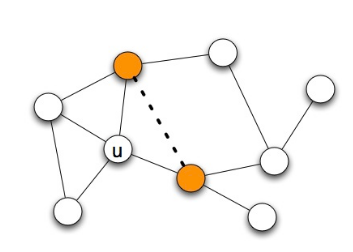
\includegraphics[width=.45\columnwidth]{push}} \quad
	\subfloat[Two-hop walk]{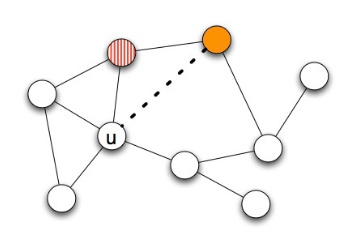
\includegraphics[width=.45\columnwidth]{pull}\label{fig:ipsum}}
	\caption[Discovery Methods]{Discovery Methods} % The text in the square bracket is the caption for the list of figures while the text in the curly brackets is the figure caption
	\label{fig:esempio}
\end{figure}
We are interested in studying the time taken by process to converge to the transitive closure of the graph.
\subsection{Notation}

\begin{table}[hbt]
	\caption{Table of Notations}
	\centering
	\begin{tabular}{llr}
		\cmidrule(r){1-2}
		Notation & Description \\
		\midrule
		$\delta_t$ & Minimum degree of $G_t$  \\
		$N_t^i(u)$ & Set of nodes at distance $i$ from $u$ in $G_t$ \\
		$d_t(u)$ & Degree of $u$ in $G_t$ \\
		$d_t(u, S)$ & Degree induced on $S$ \\
		\bottomrule
	\end{tabular}
	\label{tab:label}
\end{table}

\subsection{Useful lemmas}

\begin{lemma}\label{lem:1}
	$|\cup_{i=1}^{4} N_t^i(u)| \geq min \{ 2\delta_t, n-1\}$ for all $u \in G_t$.
\end{lemma}
\begin{proof}
	If $N_t^3 \ne \emptyset$, then $|\cup_{i=2}^{4} N_t^i(u)| \geq \delta_t$ and $|N_t^1(u) \geq \delta_t$. So $|\cup_{i=1}^{4} N_t^i(u)| \geq 2\delta_t$ since the two sets are disjoint. \\
	If $N_t^3 = \emptyset$, $N_t^1(u) \cup N_t^2(u) = n-1$ since $G_t$ is connected.
\end{proof}

\begin{lemma}\label{lem:2}
	Consider $k$ Bernoulli experiments in which the success probability of the $ith$ experiment is at least $i/m$ where $m \geq k$. If $X_i$ denotes the number of trials needed for experiment $i$ to output a success and $X = \sum_{i=1}^{k}X_i$, then $Pr[X > (c+1)m\ln m] < \frac{1}{m^c}$.
\end{lemma}
\begin{proof}
	w.l.o.g assume that $k=m$. The problem can be seen as \textit{coupon collector problem} where $X_{m+i-1}$ is the number of steps to collect $ith$ coupon. Consider the probability of not obtaining the $ith$ coupon after $(c+1)m\ln m$ steps, we have:
	\begin{math}
		(1 - \frac{1}{m})^{(c+1) m \ln m} < e^{-(c+1)\ln m} = \frac{1}{m^{c+1}}
	\end{math}
	By union bound, the probability that some coupon has not been collected after $(c+1)m \ln m$ steps is less than $\frac{1}{m^c}$.
\end{proof}

%----------------------------------------------------------------------------------------
%	METHODS
%----------------------------------------------------------------------------------------

\section{Triangulation Results}
\subsection{Upper Bound}
\subsection{Lower Bound}

\begin{theorem}[Upper bound for triangulation process]\label{thm:3}
	For any connected undirected graph, the triangulation process converges to a complete graph in $O(n \log^2 n)$ rounds with high probability.
\end{theorem}
In order to prove Theorem \ref{thm:3}, we prove that the minimum degree of the graph increases by a constant factor (or equals to $n-1$) in $O(n\log n)$ steps. We say that a node $v$ is \textbf{weakly tied} to a set of nodes $S$ if $d_t(v, S) < \delta_0 / 2$, and \textbf{strongly tied} to a set of nodes $S$ if $d_t(v, S) \geq \delta_0 / 2$.

\begin{lemma}\label{lem:4}
	If $d_t(u) < \min \{n-1, (1+\frac{1}{4} \delta_0)\} $ and $w \in N_t^1(u)$ has at least $\frac{\delta_0}{4}$ edges to $N_t^2(u)$, then the probability that $u$ connects to a node in $N_t^2(u)$ through $w$ in round $t$ is at least $\frac{1}{6n}$.
\end{lemma}
\begin{proof}
	The probability that $u$ connects to a node in $N_t^2(u)$ through $w$ in round $t$ is: \\
	\begin{center}
	\begin{math}
		\frac{d_t(w, N_t^2(u))}{D_t(w)} \times \frac{1}{d_t(w)} \geq
		\frac{d_t(w, N_t^2(u))}{D_t(w)} \times \frac{1}{n} \geq
		\frac{d_t(w, N_t^2(u))}{|N_t^1(u)|+ d_t(w, N_t^2(u))} \times \frac{1}{n} \geq
		\frac{d_t(w, N_t^2(u))}{(1 + \frac{1}{4})\delta_0 + d_t(w, N_t^2(u))} \times \frac{1}{n} \geq
		\frac{ \frac{\delta_0}{4} }{(1 + \frac{1}{4})\delta_0 + \frac{\delta_0}{4}} \times \frac{1}{n} =
			\frac{1}{6n}
	\end{math}
	\end{center}
\end{proof}

\begin{lemma}\label{lem:5}
	If $d_t(u) < \min \{n-1, (1+\frac{1}{4} \delta_0)\} $ and $w \in N_t^1(u)$ is weakly tied to $N_t^2(u)$, and $v \in N_0^2(u) \cap N_0^1(w)$, then $u$ connects to $v$ through $w$ in round $t$ with probability at least $\frac{1}{4\delta_0^2}$.
\end{lemma}
\begin{proof}
	Since $w$ is weakly tied to $N_t^2(u)$ and $d_t(w)$ is at most $|N_t^1(u)|+ d_t(w, N_t^2(u))$, we obtain that $d_t(w)$ is at most $(1 + \frac{1}{4})\delta_0 + \frac{\delta_0}{2}$. Therefore, the probability that $u$ connects to $v$ through $w$ in round $t$ equals:
	\begin{center}
		\begin{math}
			\frac{1}{d_t(w)^2} \geq
			\frac{1}{((1 + \frac{1}{4})\delta_0 + \frac{\delta_0}{2})^2} \geq
			\frac{1}{\frac{7\delta_0}{4}^2} \geq
			\frac{1}{4\delta_0^2}.
		\end{math}
	\end{center}
\end{proof}
To analyze the growth in the degree of a node $u$, we consider two overlapping cases. The first case is when more than $\delta_0/4$ nodes of $N_t^1(u)$ are strongly tied to $N_t^2(u)$, and the second is when less than $\delta_0/3$ nodes of $N_t^1(u)$ are strongly tied to $N_t^2(u)$. 


\begin{lemma}[Several nodes are strongly tied to two-hop neighbors]\label{lem:6}
	There exists a $T = O(n \log n)$ such that if more than 
\end{lemma}
%------------------------------------------------

\subsection{Paragraphs}

\lipsum[6] % Dummy text

\paragraph{Paragraph Description} \lipsum[7] % Dummy text

\paragraph{Different Paragraph Description} \lipsum[8] % Dummy text

%------------------------------------------------

\subsection{Math}

\lipsum[4] % Dummy text

\begin{equation}
\cos^3 \theta =\frac{1}{4}\cos\theta+\frac{3}{4}\cos 3\theta
\label{eq:refname2}
\end{equation}

\lipsum[5] % Dummy text

\begin{definition}[Gauss] 
To a mathematician it is obvious that
$\int_{-\infty}^{+\infty}
e^{-x^2}\,dx=\sqrt{\pi}$. 
\end{definition} 

\begin{theorem}[Pythagoras]
The square of the hypotenuse (the side opposite the right angle) is equal to the sum of the squares of the other two sides.
\end{theorem}

\begin{proof} 
We have that $\log(1)^2 = 2\log(1)$.
But we also have that $\log(-1)^2=\log(1)=0$.
Then $2\log(-1)=0$, from which the proof.
\end{proof}

%----------------------------------------------------------------------------------------
%	RESULTS AND DISCUSSION
%----------------------------------------------------------------------------------------

\section{Results and Discussion}

Reference to Figure~\vref{fig:gallery}. % The \vref command specifies the location of the reference

\begin{figure}[tb]
\centering 
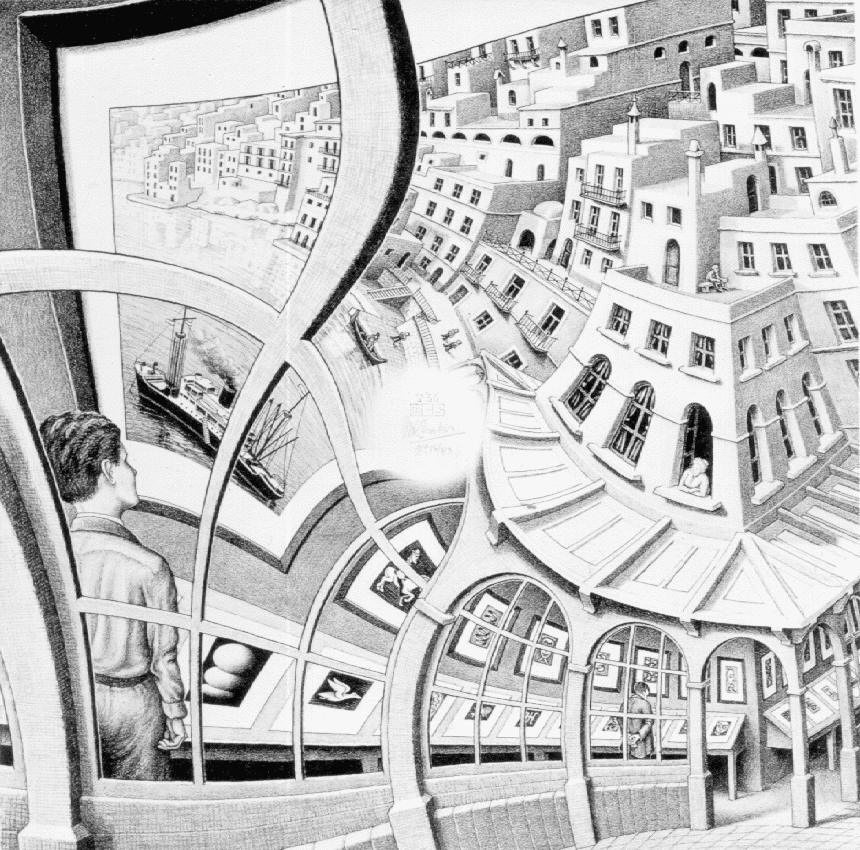
\includegraphics[width=0.5\columnwidth]{GalleriaStampe} 
\caption[An example of a floating figure]{An example of a floating figure (a reproduction from the \emph{Gallery of prints}, M.~Escher,\index{Escher, M.~C.} from \url{http://www.mcescher.com/}).} % The text in the square bracket is the caption for the list of figures while the text in the curly brackets is the figure caption
\label{fig:gallery} 
\end{figure}

\lipsum[10] % Dummy text

%------------------------------------------------

\subsection{Subsection}


\subsubsection{Subsubsection}



\begin{description}
\item[Word] Definition
\item[Concept] Explanation
\item[Idea] Text
\end{description}


\begin{itemize}[noitemsep] % [noitemsep] removes whitespace between the items for a compact look
\item First item in a list
\item Second item in a list
\item Third item in a list
\end{itemize}



Reference to Table~\vref{tab:label}. % The \vref command specifies the location of the reference

%------------------------------------------------

\subsection{Figure Composed of Subfigures}

Reference the figure composed of multiple subfigures as Figure~\vref{fig:esempio}. Reference one of the subfigures as Figure~\vref{fig:ipsum}. % The \vref command specifies the location of the reference

\lipsum[15-18] % Dummy text

\begin{figure}[tb]
\centering
\subfloat[A city market.]{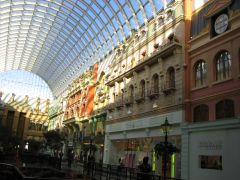
\includegraphics[width=.45\columnwidth]{Lorem}} \quad
\subfloat[Forest landscape.]{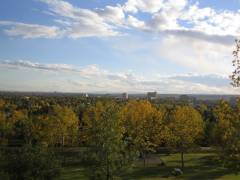
\includegraphics[width=.45\columnwidth]{Ipsum}\label{fig:ipsum}} \\
\subfloat[Mountain landscape.]{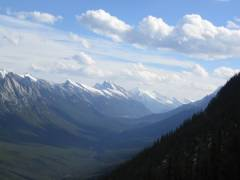
\includegraphics[width=.45\columnwidth]{Dolor}} \quad
\subfloat[A tile decoration.]{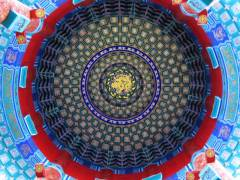
\includegraphics[width=.45\columnwidth]{Sit}}
\caption[A number of pictures.]{A number of pictures with no common theme.} % The text in the square bracket is the caption for the list of figures while the text in the curly brackets is the figure caption
\label{fig:esempio}
\end{figure}

%----------------------------------------------------------------------------------------
%	BIBLIOGRAPHY
%----------------------------------------------------------------------------------------

\renewcommand{\refname}{\spacedlowsmallcaps{References}} % For modifying the bibliography heading

\bibliographystyle{unsrt}

\bibliography{sample.bib} % The file containing the bibliography

%----------------------------------------------------------------------------------------

\end{document}